% Fair topics for CS340 MIDTERM:
% \begin{enumerate}
%     \item test vs. training
%     \item decision trees
%     \item decision stumps
%     \item naive Bayes
%     \item k-nn
%     \item ensemble methods
%     \item clustering
%     \item outlier detection
%     \item least squares
%     \item norms
%     \item change of bases (polynomial bases)
%     \item log-sum-exp
%     \item huber
%     \item gradient descent
%     \item linear 
%     \item nearest neighbors
%     \item k-means clustering
%     \item naive Bayes
%     \item Probabilistic classification
%     \item cross validation
% \end{enumerate}

\documentclass{article}

\usepackage{fullpage}
\usepackage{color}
\usepackage{amsmath}
\usepackage{url}
\usepackage{verbatim}
\usepackage{graphicx}
\usepackage{parskip}
\usepackage{amssymb}
\usepackage{amsfonts}
\usepackage{nicefrac}
\usepackage{listings} % For displaying code
\usepackage{algorithm2e} % pseudo-code
\usepackage{natbib}
\usepackage{todonotes}

% Answers
\def\rubric#1{\gre{Rubric: \{#1\}}}{}

% Colors
\definecolor{blu}{rgb}{0,0,1}
\def\blu#1{{\color{blu}#1}}
\definecolor{gre}{rgb}{0,.5,0}
\def\gre#1{{\color{gre}#1}}
\definecolor{red}{rgb}{1,0,0}
\def\red#1{{\color{red}#1}}
\def\norm#1{\|#1\|}

% Math
\def\R{\mathbb{R}}
\def\argmax{\mathop{\rm arg\,max}}
\def\argmin{\mathop{\rm arg\,min}}
\newcommand{\mat}[1]{\begin{bmatrix}#1\end{bmatrix}}
\newcommand{\alignStar}[1]{\begin{align*}#1\end{align*}}
\def\half{\frac 1 2}

% LaTeX
\newcommand{\fig}[2]{\includegraphics[width=#1\textwidth]{#2}}
\newcommand{\centerfig}[2]{\begin{center}\includegraphics[width=#1\textwidth]{#2}\end{center}}
\def\items#1{\begin{itemize}#1\end{itemize}}
\def\enum#1{\begin{enumerate}#1\end{enumerate}}

\begin{document}

\title{CPSC 340 Machine Learning Take-Home Midterm Exam\\ (Fall 2020)}
\date{}
\maketitle
\vspace{-5em}

%     \item test vs. training
%     \item decision trees
%     \item decision stumps
%     \item naive Bayes
%     \item k-nn
%     \item ensemble methods
%     \item clustering
%     \item outlier detection
%     \item least squares
%     \item norms
%     \item change of bases (polynomial bases)
%     \item log-sum-exp
%     \item huber
%     \item gradient descent
%     \item linear 
%     \item nearest neighbors
%     \item k-means clustering
%     \item naive Bayes
%     \item Probabilistic classification
%     \item cross validation


\section*{Instructions}
This is a take home midterm with two components:\enum{
	\item an individual component 
	\item a group component for groups of up to 5.  Note that your final and midterm groups will not be allowed to have any overlap in membership besides you.
%	\item and an optional/extra credit component for groups of up to 5.
}

You may work on the group components as an individual, but it is to your advantage to team up with others. There will be no leniency in grading for smaller groups or individual work. \\
% If you decide to work on the optional question 3, you must do so \textit{with the same group} as for question 2. Please take time at the start to discuss among group members on the plan of approach for this final.

\subsection*{Submission instructions}
\textit{Typed}, \LaTeX-formatted solutions are due on Gradescope by \textbf{Monday, October 26}.\items{
	\item You must use the latex skeletons provided later in this document to format your reports.  You may include additional, terse, comments in additional sections beyond those specified.
	\item Each student must submit question 1 individually as a pdf file named \texttt{question1.pdf}. Include your CS ID and student ID. Upload your answer on Gradescope under \textbf{Midterm Exam Question 1}.
	\item Each group should designate one group member to submit their solution to question 2 to Gradescope using its group feature (\url{https://www.gradescope.ca/help#help-center-item-student-group-members}). Please hand in your work separately for question 2 on Gradescope. Submit a pdf file named \texttt{question2.pdf} containing all of your answers and code for question 2 under \textbf{Midterm Exam Question 2}. Include each group members' CS IDs and student IDs.}

\section*{Question 1 - Individual \hspace{7.0cm}[70/100 points]}

In this question, you are provided with a dataset consisting of tweets from the two U.S. presidential candidates - Donald Trump, and Joe Biden. The features of each word in each tweet were extracted using the word2vec algorithm (see \url{https://en.wikipedia.org/wiki/Word2vec}; word2vec will be covered later in the term, understanding how it works is not required to be able to complete this question) then combined via averaging to form a fixed-length feature vector per tweet. Your task is to design a number of binary classifiers which, given a tweet vector, predict whether the tweet was authored by  Donald Trump or Joe Biden. You are given the following files.

\begin{itemize}
    \item \texttt{wordvec\_train.csv} - dataset of word2vec features. Each data entry has 200 numerical features, and a label (1 for Donald Trump, and 0 for Joe Biden). This is your training data.
    \item \texttt{tweet\_train.csv} - dataset of tweets prior to feature extraction (you don't need to use this, it is provided just for own amusement). These correspond to features in your training data.
    \item \texttt{wordvec\_test.csv} - dataset of word2vec features. This is your test set.
    \item \texttt{tweet\_test.csv} - tweets corresponding to test set features.
\end{itemize}


You will implement the following classifiers.

\begin{enumerate}
    \item A random forest classifier.
    \begin{enumerate}
        \item Which uses the Gini index as a splitting score.
        \item Where the K-means algorithm is used to quantize each feature, determining the thresholds to search over for each feature. 
    \end{enumerate}
    \item Naive Bayes for continuous features.
    \item K nearest neighbours with cosine similarity as the distance metric.
    \item A stacking ensemble consisting of your classifiers from parts 1-3, where a decision tree is used as a meta-classifier.
\end{enumerate}

All of these concepts are familiar to you and have been introduced in class.  As the details of these specific models are ``new'' to you, we elaborate on them in the following sections. %Please fill in your answers in the provided \texttt{.tex} file.

\subsection*{Gini Impurity and Gini index}

Gini Impurity measures the probability of misclassifying an observation. Consider a classification problem with $J$ classes. Let $p_i$ be the fraction of items labeled with class $i$ at a given node. Then the Gini impurity at the node is given by,

\begin{equation}
\mathbf {Gini\: Impurity} = G(p_1, \ldots, p_J) = \sum_{i =1}^J p_{i}(1-p_{i}).
\end{equation}

% where J is the number of classes, and $p_i$ is the fraction of items labeled with the class $i$. The lower the Gini Impurity, the lower the likelihood of misclassification.

The \textbf{Gini\:Index} is the weighted sum of Gini Impurity for a split in our data. Let $p_i^{\ell}$ be the fraction of items labeled with class $i$ in the left side of our split, and $p_i^{r}$ be the fraction of items labeled with class $i$ in the right side of our split. Moreover, if we take $N_{t}$ to be the total number of data, then $N_{r}$ is the number of data in the right side of the split, and $N_{\ell}$ is the number of data in the left side of the split. In the end, the Gini Index of the split is given by,

\begin{equation}
\mathbf{Gini\: Index} = \frac{N_{\ell}}{N_{t}}\:G(p_1^{\ell}, \hdots, p_J^{\ell}) + \frac{N_{r}}{N_{t}}\:G(p_1^r, \hdots, p_J^r).
\end{equation}

Finally, we can use the Gini index as a splitting criteria in a decision tree. To do that, first we need to find the split with the minimum Gini index between the set of all the possible splits for each feature. If the minimum Gini index was less than the Gini impurity of the data before the split, then we select the split with the minimum Gini index as the decision rule, otherwise we stop splitting. For more information please see the appendix at the end of this file. 


\subsection*{Using K-means to determine thresholds}
K-means can be used as a binning algorithm for continuous data. For each feature, you must train a separate instance of k-means. When you are creating your decision tree splits, instead of searching over every possible unique value in the data, you should only consider splitting at each of the k means-derived thresholds.

\subsection*{Continuous Naive Bayes}

In our description of Naive Bayes thus far we have only seen it used for problems with discrete features. However, we can use Naive Bayes for continuous features by assuming that for each class, each feature comes from some continuous distribution. For now, we will make the assumption that each of the features come from an univariate normal distribution.  Note that the class conditional independence assumption made in the lectures resulted in computing the product of Bernoulli likelihoods in the decision rule.  Here the class conditionally independent likelihoods will be univariate Gaussian likelihoods.

The univariate Gaussian likelihood, or normal distribution,  has two parameters - the mean $\mu$, and the standard deviation $\sigma$, of the distribution,
\begin{equation}   
    p(x \mid \mu, \sigma) = \frac{1}{\sigma \sqrt{2\pi}}\exp\left(-\frac{1}{2}\left(\frac{x - \mu}{\sigma}\right)^2\right).
\end{equation}

In Naive Bayes, given a data-label pair $(x_i, y_i)$, we construct and then make predictions using the quantity,
\begin{equation}   
    p(x_i \mid y_i = y_c),
\end{equation}
where $y_c$ is an arbitrary class label. In the continuous case, for the class $c$, for each feature $d$, we would have a normal distribution with parameters $\mu_{c}^d, \sigma_{c}^d$. We also let $x_i^d$ denote the $d$th feature of data entry $x_i$. Thus, we make predictions with the following quantity,
\begin{equation}\label{likelihood}    
p(x_i \mid y_i = y_c) = \prod_d p(x_{i}^d \mid \mu_{c}^d, \sigma_{c}^d),
=\prod_d \left( \frac{1}{\sigma_c^d \sqrt{2\pi}}\exp\left(-\frac{1}{2}\left(\frac{x_i^d - \mu_c^d}{\sigma_c^d}\right)^2\right)\right).
\end{equation}
% \begin{equation}   
%     p(x_i \mid y_i = y_c) = \prod_d p(x_{i,d} \mid \mu_{c,d}, \sigma_{c,d}^2, y_{i} = y_{c}).
% \end{equation}

In order to estimate $\mu_{c,d}, \sigma_{c,d}^2$ from the data, we make a maximum likelihood assumption. For the normal distribution, this amounts to estimating the mean and the variance of each feature for both classes, and using these parameters to make predictions.

Recall that the maximum likelihood estimators for the mean and variance of the univariate Gaussian distribution are
\begin{align*}
    \mu_{c}^d &= \frac{1}{n_c} \sum_{i=1}^{n_c} x_i^d \\
    (\sigma_{c}^d)^2 &= \frac{1}{n_c} \sum_{i=1}^{n_c}\left(\mu_c^d - x_i^d \right)^2. 
\end{align*}

\emph{Hint:} When multiplying many small probabilities together as in \eqref{likelihood}, the product can go to zero very quickly. Instead, you should make your predictions in log space,
\begin{align}
    \log\left(p(x_i \mid y_i = y_c)\right) = -\sum_{d} \left(\frac{1}{2}\left(\frac{x_i^d - \mu_c^d}{\sigma_c^d}\right)^2 + \log\left( \sigma_c^d \sqrt{2\pi} \right)\right).
\end{align}

\subsection*{Cosine similarity}

Cosine similarity measures the similarity between two vectors. It is measured by the cosine of the angle between two vectors and determines whether two vectors are pointing in roughly the same direction,
\begin{equation}
 Similarity(x_i, x_q)  = \frac{x_{i}^T x_{q}}{\norm{x_{i}}\norm{x_{q}}}.
\end{equation}


\subsection*{Stacking classifier}

 Stacking is an ensembling technique that combines multiple classifiers via a meta-classifier. The individual classifiers are trained on the original training data with their individual losses and learning algorithms. Then, the meta-classifier uses the predictions of the classifiers in the ensemble as features and is trained with those as inputs and the ultimate output as its output. For more information see slide 26 in Lecture 7.
 



\section*{Question 2 - Group \hspace{8.1cm}[30/100 points]}

This part of the midterm is a group project that takes place on Kaggle.  There are two phases to this competition which come in the form of two essentially identical (but spaced in time) Kaggle competitions.  The Phase 1 Kaggle competition is at \url{https://www.kaggle.com/t/dd5029ad34d14b1eb9791aaeba0a09fd}.  The Phase 2 Kaggle competition is at \url{https://www.kaggle.com/t/b94ffde05677429c848b6517c9e37d2b}. You can sign up for a new account or use an existing one; however, note that the Kaggle servers may be in the US, so bear this in mind.  We recommend that for data protection purposes you use a non-identifiable (but ideally hilarious) team name.  You will link your group members to your team name in your submission document.

You are only allowed to use linear regression techniques to solve this problem.  No neural networks, support vector machines, etc.  You are not allowed to use any software that you did not develop yourself.  There is one exception to this: you may use homework support code and code you wrote yourself for your homeworks.

Your mark for this part of the midterm will be based on the score from Kaggle for your Phase 2 test set predictions (see below and the Kaggle competitions pages), a written report that explains your findings, and your code. Your report must \LaTeX formatted and follow the format given in the answer template for Question 2 below.

The problem you are tasked with in the Kaggle competitions is predicting ``forward in time'' five days of Covid-19 daily death counts for the entire country of Canada. The ultimate evaluation of your model's performance will only happen {\em after} the test submission deadline.

Here's how it is going to work.  The competition will proceed in two phases.   In the first phase competition we will provide you with an {\em initial training dataset} dataset consisting of 4 different Covid-19-related counts for effectively all countries in the world for all days starting from Dec.~31st, 2019 up to Oct.~5th, 2020 when the initial prediction window starts.  The Phase 1 Kaggle competition will be configured to allow you to upload {\em initial test predictions} consisting of the Canadian daily Covid-19 death totals for the days Oct.~6-16th, 2020.  In the second phase competition we will provide you, {\em  on the day before the midterm is due}, with a {\em second training dataset} that runs up to the 25th of Oct.  You will then be tested, after the exam is handed in 
(Oct.~26th is the due date) on 5 days of predictions (Oct.~26th, 27th, 28th, 29th, and 30th) of daily Canadian Covid-19 daily death counts.  Your test accuracy will be measured (and compared) in terms of means squared error against the actual deaths that happen on those days.\footnote{yes, this means that this question and your performance won't be known until several days after your midterm is handed in and your {\em static} predictions have already been made}

You are free to construct any feature set you wish and train as many linear regression models as you want in order to solve this task.  Here and below we provide some useful guidance about how to use linear regression models to learn one-step-ahead prediction models that ``eat their own predictions.''

\subsection*{Linear Autoregressive Models}

To start, consider a one-dimensional time series dataset $D$ consisting of values $[d_1, d_2, d_3, \ldots, d_t, \ldots, d_T]$.  A linear regression model for one-step-ahead prediction can be learned by constructing

\begin{align*}
y &= \begin{bmatrix}
d_K \\ d_{K+1}\\ \vdots\\ d_T
\end{bmatrix} &\qquad
X &= 
\begin{bmatrix}
x_K^T \\
x_{K+1}^T \\
\vdots \\
x_{T}^T \\
\end{bmatrix}
 =
\begin{bmatrix}
1 & d_1 & d_2 & \cdots & d_{K-1}\\
1 & d_2 & d_3 &  \cdots & d_{K}\\
\vdots & \cdots &\cdots &\cdots &\vdots\\
1 & d_{T-K} & d_{T-K+1} &  \cdots & d_{T-1}\\
\end{bmatrix}.	
\end{align*}

Here we have implicitly defined feature vectors $x_i$ which correspond to the vector of $K$ previous values in $D$ used to predict $y_i.$
If you learn a regression model with parameter vector $w$ with this data you can use it to predict ${\hat y}_{T+1}$ given ${\tilde x}_{T+1} = [1,\; d_{T-K+1},\; d_{T-K+2},\;  \ldots,\;  d_{T}]^T$. This is what is known as an ``autoregressive'' model.  What is more, such a model can be used to make multi-step predictions into the future by continuing the following recursion 
\begin{align*}
    {\hat y}_{T+2} \approx [1,\; d_{T-K+2},\; d_{T-K+3},\;  \ldots,\;  d_{T},\; {\hat y}_{T+1}]w
\end{align*}
where the latest prediction is fed into the feature vector in the appropriate position.

\subsection*{Prediction Task}



In this competition you only need to make predictions about Canadian daily death counts.  However, the performance of your submission will largely be dictated by how you make use of the other features in the data, particularly the counts in other countries at the same time.  
The data you receive we call $D.$ It consists of a number of $\{\mathrm{country\_id,	date, cases, deaths, cases\_14\_100k, cases\_100k}\}$ tuples.  An exact explanation of these features is available online.\footnote{\url{https://www.ecdc.europa.eu/en/publications-data/download-todays-data-geographic-distribution-covid-19-cases-worldwide}}

% Let $\mathcal{C} = \{AD, AE, \ldots, CA, \ldots ZW\}$ be the set of unique country codes in $D$.  Let $\mathcal{D} = \{31/1/19, \ldots, 10/9/20\}$ be the set of dates in $D$. 
The simplest thing you could try is the regression model just described, trained and operating only on the Canadian daily death counts. Of course it is also clear that you could build independent country- and ``feature''-specific regressors
(by feature here we mean colloquially the cases, deaths, cases\_14\_100k, cases\_100k values).   This, unfortunately, would not leverage count values from other countries in making the country and feature specific predictions.  

This challenge problem gets much more interesting when you think about ways to leverage all the additional data available from countries around the world, particularly by designing feature matrices for each regressor that leverages data from other countries, either in aggregate or in specific. 

Here is one kind of thing that you can do.  Call the output that we wish to predict  for a particular feature (take cases for example), day (take 8/21/20 for example), and country (take AD for example) combination $y_i.$  The feature vector you construct for this particular instance can carry information from all countries on any days prior to 8/21/20.  These can be aggregated features, can be restricted to neighboring countries, or countries with high flight connectivity, etc.  

Moreover, depending on how you construct your feature space, you can build models that are not specific to a particular country.  So long as the first, say, $L$ entries of your feature vector are extracted from the data from the country of the required prediction on any days prior and the remaining $d-L$ entries are features extracted from the data from all countries on any days prior the resulting regression model will be country-agnostic.

\begin{figure}[tbph]
    \centering
    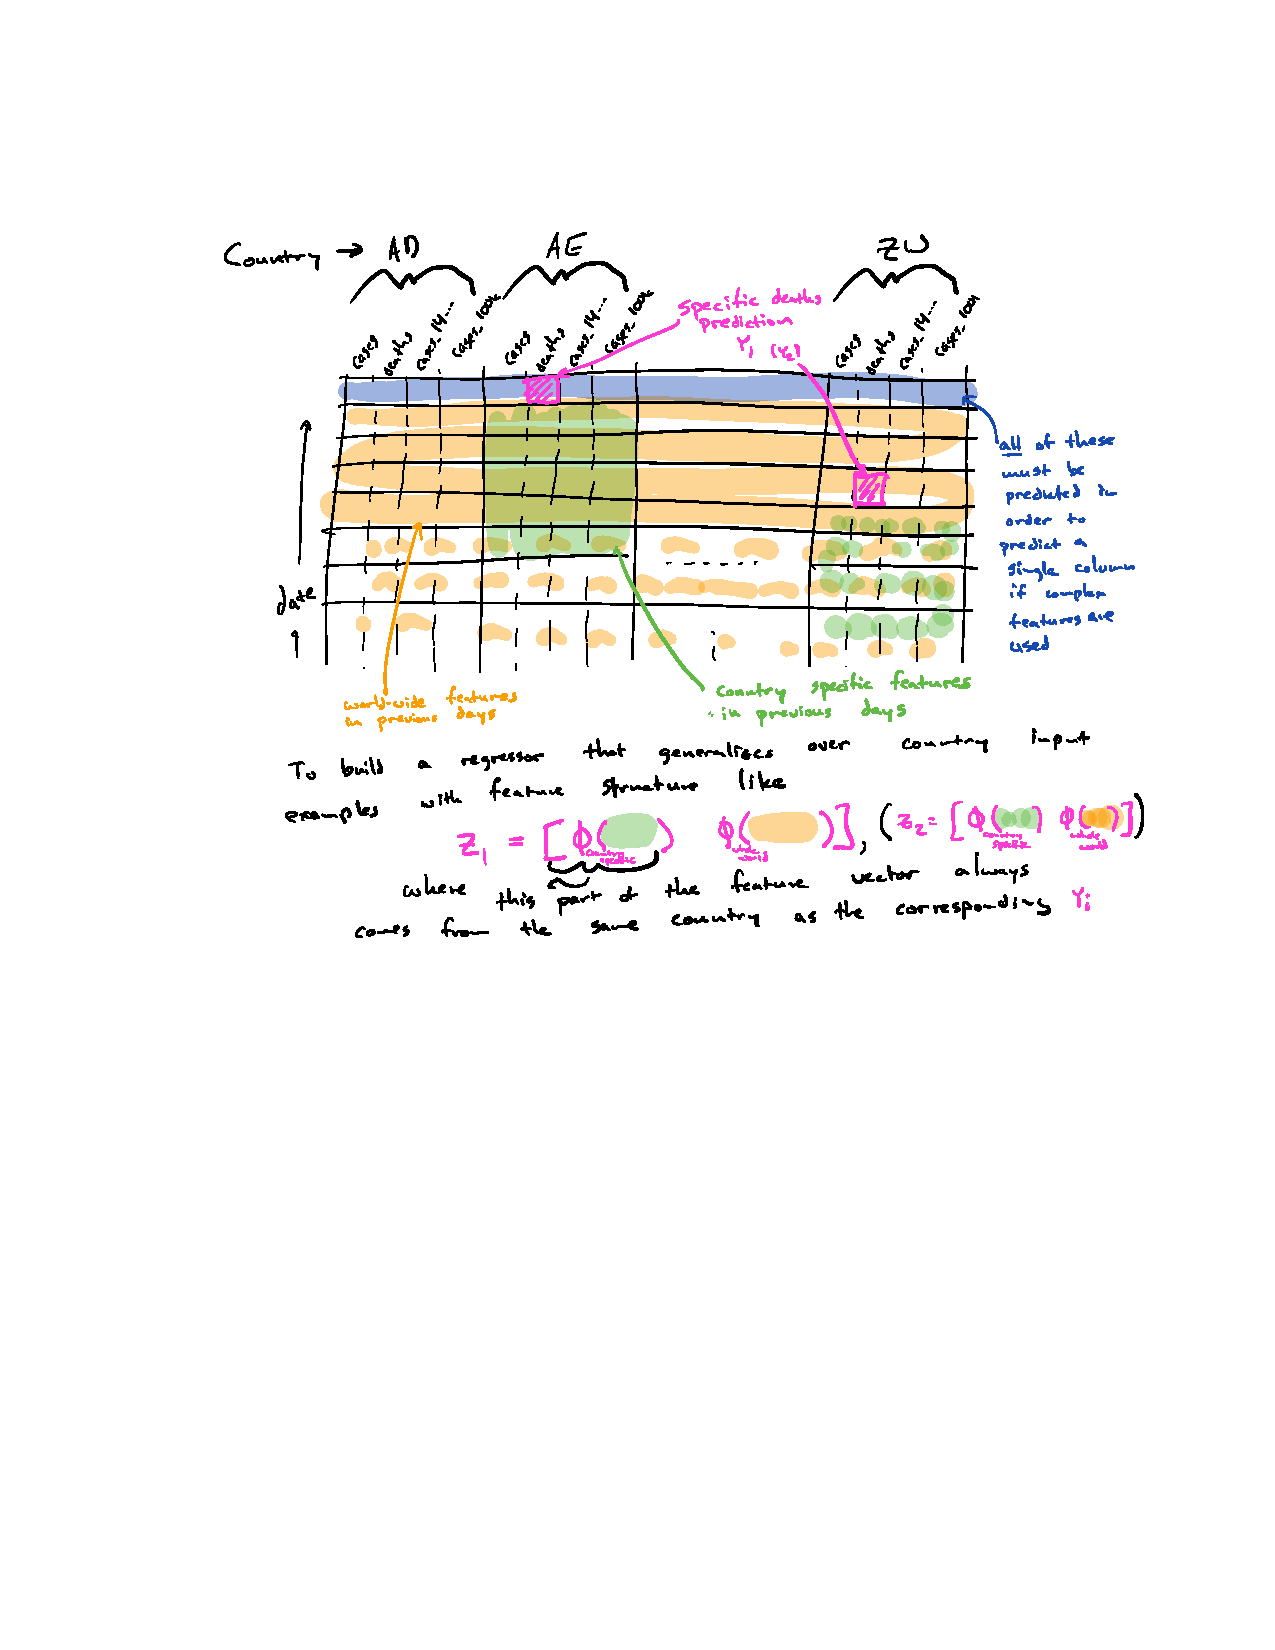
\includegraphics[width=1.0\textwidth]{../figs/midtermfeaturediagram.pdf}
    \caption{Feature Matrix Hints Diagram}
    \label{fig:midtermfeaturediagram}
\end{figure}


See Fig~\ref{fig:midtermfeaturediagram} for helpful hints about how one might construct such complex and informative feature spaces.

\subsection*{Submitting Your Results}


You need to be prepared to do several things.  First, as usual, you must bundle your code along with a \texttt{.pdf} generated from the filled in \LaTeX report skeleton into a \texttt{.zip} file and submit it to Gradescope. Again, marks may be taken off for very messy or hard to read code, so make sure to use descriptive variable names and include comments where appropriate.

Also, Phase 2 of the Kaggle competition will be released the day before the midterm is due.  You may retrain your model on the additional data or you may simply use it as input to predict five days into the future past the midterm due date.  You will upload these predictions to the Kaggle server and your model's relative test performance will be made available in 5 days time. 



\newpage
%%%%%%%%%%%%%%%%%%%%%%%%%%%%%%%%%%%%%%%%%%%%%%
% LaTeX answer format skeleton
%
% Delete everything above here (except, of course, for the document
% preamble).  You will need to separate the following into 3
% different latex files.
%
% To write up your answers for submission, please 
% odify everything below here as required.  Reminder _3_ different
% .pdf's are to be submitted.  
% The names of these pdf's should be as stated at the beginning of the
% exam: question1.pdf, question2.pdf, question3.pdf
%%%%%%%%%%%%%%%%%%%%%%%%%%%%%%%%%%%%%%%%%%%%%%
\section*{Template for Question 1}

\setcounter{section}{0}


\section{Individual Classifiers}

\subsection{Result}

Report the train and test result for each classifier in the given table. You should use the following hyperparameters,
\begin{enumerate}
    \item Random Forest: no max cap on depth, and a forest size of 15 trees.
    \item KNN: $k=3$.
    \item Continuous Naive Bayes: has no hyperparameters.\\
\end{enumerate}

\begin{center}
 \begin{tabular}{|c | c | c|} 
 \hline
 Model & Your Train Error (\%) & Your Test Error (\%) \\ [0.5ex]
 \hline\hline
 Random Forest & & \\
 KNN & & \\
 Naive Bayes &  & \\
 
 \hline
\end{tabular}\\~\\~\\
\end{center}

Explain in one paragraph why you think a particular classifier works better on this dataset.\\~\\~\\~\\

\subsection{Code}
Include the code you have written for each particular classifier.
\begin{enumerate}
\item Random Forest\\
\item KNN\\
\item Naive Bayes\\
\end{enumerate}

\section{Stacking}

% In this section, we are going to implement a stacking ensemble. Ensebmle the classifiers from the previous section, and use a decision tree which uses their predictions as inputs to make decision. 

% \subsection{Choice of classifiers}
% Write the information of the models (and the hyper-parameter of each model) that you selected for each classifier.

% \begin{enumerate}
% \item Classifier 1\\
% \item Classifier 2\\
% \item Classifier 3\\
% \item Meta Classifier\\
% \end{enumerate}

\subsection{Result}

Report the test error and training error of the stacking classifier.\\~\\~\\~\\

\subsection{Code}

Include all the code you have written for stacking classifier

% \begin{enumerate}
% \item Classifier 1\\
% \item Classifier 2\\
% \item Classifier 3\\
% \item Meta Classifier\\
% \end{enumerate}


\newpage

\section*{Template for Question 2}
\setcounter{section}{0}

\section{Team}
\begin{tabular}{|c | c |} 
\hline
Team Members & \emph{all team member names and csids here} \\
\hline
Kaggle Team Name & \emph{your Kaggle team name here}\\
\hline
\end{tabular}
\section{Solution Summary}
\emph{In no more than several paragraphs summarize the approach you took to address the problem.}
\section{Experiments}
\emph{In this section report, in less than two pages, describe in technical terms the training procedures you used, including how you went about feature selection, hyperparameter value selection, training, and so forth.  Plots related to hyperparameter sweeps and other reportable aspects of your training procedure would be appreciated.}



\section{Results}

\begin{center}
 \begin{tabular}{|c | c | c |} 
 \hline
 Team Name & Kaggle Phase 1 Score & Kaggle Phase 2 Score  \\ [0.5ex]
 \hline\hline
 \emph{the name of your team} & \emph{your Phase 1 Kaggle score}  & \emph{your Phase 2 Kaggle score}  \\
 \hline
\end{tabular}
\end{center}

\section{Conclusion}
\emph{Describe what you learned and what you would have done were you to have been given more time in a few paragraphs.}
\newpage



\section*{Appendix}

\subsection*{Gini Index}

In this example, we have a dataset with two features x and y. Each data entry belongs to either the blue class or green class.

\begin{figure}[h]
	\centering
	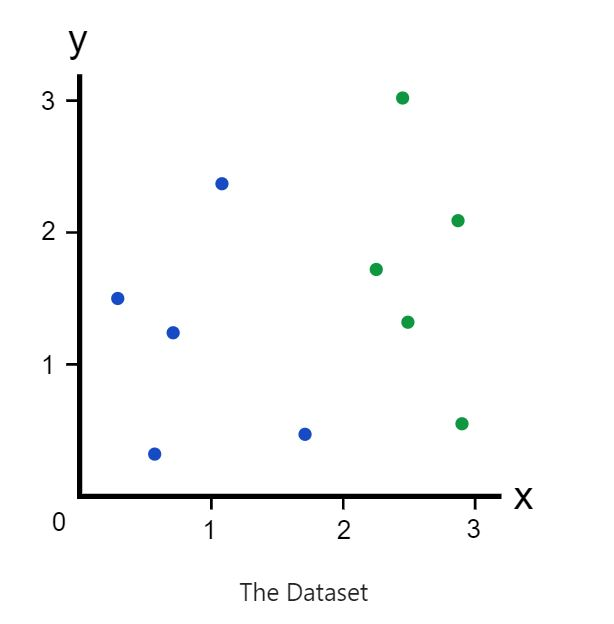
\includegraphics[scale=0.2, width=0.3\columnwidth]{../figs/gini1.JPG}
	\caption{A given dataset with two features }
	\label{}
\end{figure}



lets define\\
$p_b$ = probability of blue class,\\
$p_g$ = probability of green class.\\ \\
To compute the Gini impurity before splitting,

$G(p_g^{No Split},p_b^{No Split}) =  p_{g}^{No Split}(1- p_{g}^{No Split}) + p_{b}^{No Split}(1-p_{b}^{No Split}) = \frac{5}{10}(1 - \frac{5}{10})$,\\
$G(p_g^{No Split},p_b^{No Split}) =  \frac{1}{2}.$ \\



In order to find the best split in the x-axis, we should search over the set of possible splits. One arbitrary choice is shown in figure 2.

\begin{figure}[h]
	\centering
	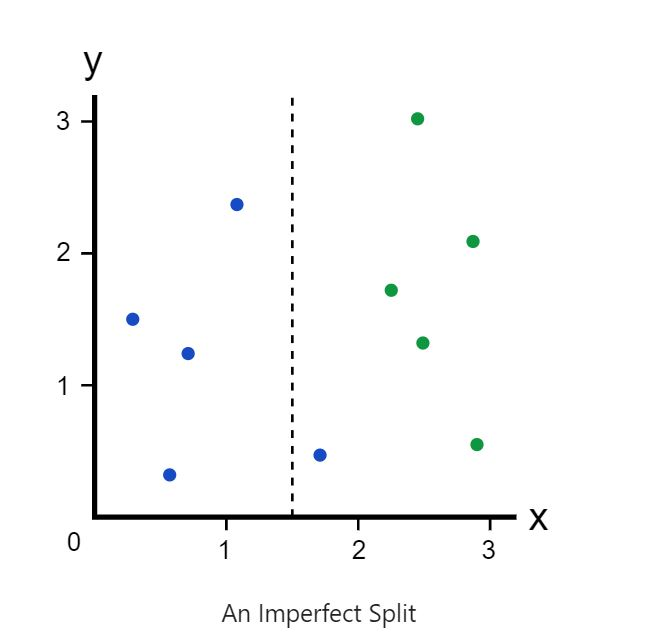
\includegraphics[scale=0.2, width=0.3\columnwidth]{../figs/gini3.JPG}
	\caption{split feature x, where x = 1.5.}
	\label{}
\end{figure}

let's compute the Gini impurity for the right side.

$G(p_g^{r},p_b^{r}) =  p_{g}^{r}(1- p_{g}^{r}) + p_{b}^{r}(1-p_{b}^{r})$, where  $p_{g}^{r} = \frac{5}{6}$ ,  $p_{b}^{r} = \frac{1}{6}$, \\ \\
 $G(p_g^{r},p_b^{r}) = \frac{10}{36}$\\


And for the left side,

$G(p_g^{l},p_b^{l}) =  p_{g}^{l}(1- p_{g}^{l}) + p_{b}^{l}(1-p_{b}^{l})$, where  $p_{g}^{l} = \frac{0}{4}$ ,  $p_{b}^{l} = \frac{4}{4}$. \\
$G(p_g^{l},p_b^{l}) = 0.$\\

In the next step, we compute the Gini index for the current split, as follosw
 
 $Gini\: Index = \frac{N_{l}}{N_{t}}*G(p_g^{l},p_b^{l}) + \frac{N_{r}}{N_{t}}*G(p_g^{r},p_b^{r})$  =$ \frac{4}{10}*0 + \frac{6}{10}*\frac{10}{36} = \frac{1}{6}.$ \\
 
Another possible split is demonstrated in the figure 3.
 
 \begin{figure}[h]
	\centering
	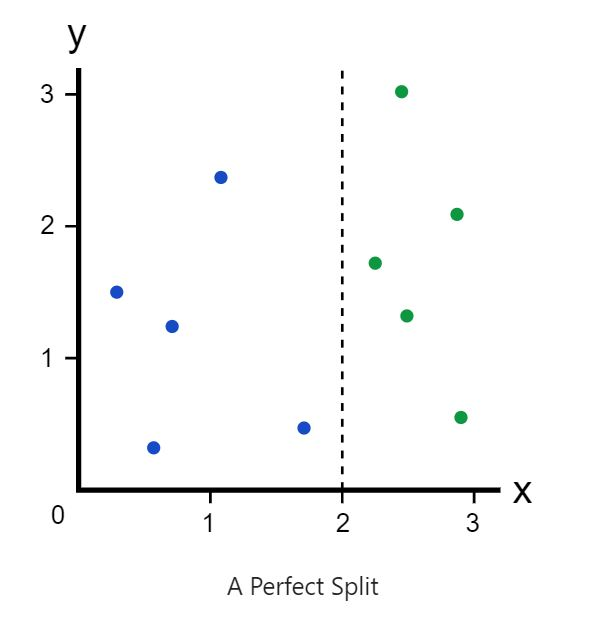
\includegraphics[scale=0.2, width=0.3\columnwidth]{../figs/gini2.JPG}
	\caption{split feature x, where x = 2. }
	\label{}
\end{figure}


To compute the Gini impurity for the right side, we have

$G(p_g^{r},p_b^{r})=  p_{g}^{r}(1- p_{g}^{r}) + p_{b}^{r}(1-p_{b}^{r})$, where  $p_{g}^{r} = \frac{5}{5}$ ,  $p_{b}^{r} = \frac{0}{5}$  \\
$G(p_g^{r},p_b^{r}) = 0.$


And the Gini impurity for the left side is

$G(p_g^{l},p_b^{l}) =  p_{g}^{l}(1- p_{g}^{l}) + p_{b}^{l}(1-p_{b}^{l})$, where  $p_{g}^{l} = \frac{0}{5}$ ,  $p_{b}^{l} = \frac{5}{5}$ \\ 
$G(p_g^{l},p_b^{l}) = 0.$

In the next step, we compute the Gini index for the current split:
 
 $Gini\: Index = \frac{N_{l}}{N_{t}}*G(p_g^{l},p_b^{l}) + \frac{N_{r}}{N_{t}}*G(p_g^{r},p_b^{r})$  =$ \frac{5}{10}*0 + \frac{5}{10}*0 = 0.$ \\

In the end, we find the minimum Gini index between the splits. The minimum Gini index for this example is when x = 2. Also, the minimum Gini index is less than Gini impurity of no split. Therefore, we select x = 2 as the splitting rule.

% \subsection*{Time Series Analysis}
% Time series data are a set of observations on the values of a variable at different times. These data are analyzed to determine the long term trend so as to forecast the future or perform some other form of analysis. In Question 2, you are going to make a time series regression model to forecast the number of COVID cases in Canada in the last 30 days, given data for all the countries. 

% To estimate a time series regression model, a trend must be estimated. You begin by creating a line chart of the time series. The line chart shows how a variable changes over time. This chart can be used to inspect the characteristics of the data, in particular, to see whether a trend exists.

% To formally test whether a linear trend occurs, run a time series regression with a time trend as the independent variable, which you can set up like so:

% \begin{equation}
% y_t = \beta_0 +\beta_1t + \epsilon_t .
% \end{equation}

% In Question 2, the dependent variable is the number of cases, and the independent variable is time (measured in days).


\end{document}
